\documentclass[11pt]{article}\usepackage[]{graphicx}\usepackage[]{color}
%% maxwidth is the original width if it is less than linewidth
%% otherwise use linewidth (to make sure the graphics do not exceed the margin)
\makeatletter
\def\maxwidth{ %
  \ifdim\Gin@nat@width>\linewidth
    \linewidth
  \else
    \Gin@nat@width
  \fi
}
\makeatother

\definecolor{fgcolor}{rgb}{0.345, 0.345, 0.345}
\newcommand{\hlnum}[1]{\textcolor[rgb]{0.686,0.059,0.569}{#1}}%
\newcommand{\hlstr}[1]{\textcolor[rgb]{0.192,0.494,0.8}{#1}}%
\newcommand{\hlcom}[1]{\textcolor[rgb]{0.678,0.584,0.686}{\textit{#1}}}%
\newcommand{\hlopt}[1]{\textcolor[rgb]{0,0,0}{#1}}%
\newcommand{\hlstd}[1]{\textcolor[rgb]{0.345,0.345,0.345}{#1}}%
\newcommand{\hlkwa}[1]{\textcolor[rgb]{0.161,0.373,0.58}{\textbf{#1}}}%
\newcommand{\hlkwb}[1]{\textcolor[rgb]{0.69,0.353,0.396}{#1}}%
\newcommand{\hlkwc}[1]{\textcolor[rgb]{0.333,0.667,0.333}{#1}}%
\newcommand{\hlkwd}[1]{\textcolor[rgb]{0.737,0.353,0.396}{\textbf{#1}}}%

\usepackage{framed}
\makeatletter
\newenvironment{kframe}{%
 \def\at@end@of@kframe{}%
 \ifinner\ifhmode%
  \def\at@end@of@kframe{\end{minipage}}%
  \begin{minipage}{\columnwidth}%
 \fi\fi%
 \def\FrameCommand##1{\hskip\@totalleftmargin \hskip-\fboxsep
 \colorbox{shadecolor}{##1}\hskip-\fboxsep
     % There is no \\@totalrightmargin, so:
     \hskip-\linewidth \hskip-\@totalleftmargin \hskip\columnwidth}%
 \MakeFramed {\advance\hsize-\width
   \@totalleftmargin\z@ \linewidth\hsize
   \@setminipage}}%
 {\par\unskip\endMakeFramed%
 \at@end@of@kframe}
\makeatother

\definecolor{shadecolor}{rgb}{.97, .97, .97}
\definecolor{messagecolor}{rgb}{0, 0, 0}
\definecolor{warningcolor}{rgb}{1, 0, 1}
\definecolor{errorcolor}{rgb}{1, 0, 0}
\newenvironment{knitrout}{}{} % an empty environment to be redefined in TeX

\usepackage{alltt}
\usepackage{amsmath}
\usepackage{stmaryrd}
\usepackage{bbm}
\usepackage{amsmath}
\usepackage{mathtools}
\usepackage{pdfpages}
\usepackage{breqn}

\newcount\colveccount
\newcommand*\colvec[1]{
        \global\colveccount#1
        \begin{pmatrix}
        \colvecnext
}
\def\colvecnext#1{
        #1
        \global\advance\colveccount-1
        \ifnum\colveccount>0
                \\
                \expandafter\colvecnext
        \else
                \end{pmatrix}
        \fi
}
\newcommand{\argmin}{\arg\!\min}

\author{Thibault Doutre, Student ID 26980469}
\title{STAT230 HW 3 \\
University of California, Berkeley}
\date{\today}
\IfFileExists{upquote.sty}{\usepackage{upquote}}{}
\begin{document}
\maketitle

\section{Theory}
\subsection{A1}

\begin{align}
E(Y|X) &= E(X\beta+\epsilon|X) \\
&= E(X\beta|X)+E(\epsilon|X) \\
&= E(X\beta|X) \\
&= X\beta
\end{align}


\begin{align}
Cov(Y|X) &= E(YY^T|X) - E(Y|X)E(Y|X)^T \\
&= X\beta \beta^T X^T - 2 E(X\beta \epsilon^T|X)+E(\epsilon \epsilon^T|X) - X\beta(X\beta)^T \\
&= -2 X\beta E(\epsilon^T|X) + E(\epsilon \epsilon^T|X) \\
&= \sigma^2 I
\end{align}

\begin{align}
\hat{\beta} &= (X^TX)^{-1}X^TY \\
&= (X^TX)^{-1}X^T(X\beta+\epsilon) \\
&= \beta + (X^TX)^{-1}X^T \epsilon 
\end{align}

Therefore: 
\begin{align}
E(\hat{\beta}|X) &= E(\beta + (X^TX)^{-1}X^T \epsilon | X) \\
&= E(\beta |X) + (X^TX)^{-1}X^T E(\epsilon | X) \\
&= \beta
\end{align}

\begin{align}
Cov(\hat{\beta}|X) &= E(\hat{\beta}\hat{\beta}^T|X) - E(\hat{\beta}|X)E(\hat{\beta}|X)^T \\
&= E((X^TX)^{-1}X^TYY^TX(X^TX)^{-1}|X) \\ 
& - E((X^TX)^{-1}X^TY)E((X^TX)^{-1}X^TY|X)^T \\
&= (X^TX)^{-1}X^T E(Y Y^T|X) X(X^TX)^{-1}-\beta \beta^T \\
&= (X^TX)^{-1}X^TX\beta \beta^T X^T X(X^TX)^{-1} \\
& +(X^TX)^{-1}X^TE(\epsilon \epsilon^T|X)X(X^TX)^{-1} -\beta \beta^T \\
&=  (X^TX)^{-1}X^T(\sigma^2 I)X(X^TX)^{-1} \\
&= \sigma^2 (X^TX)^{-1}
\end{align}

\subsection{B2}

\begin{align}
E(Y|X) &= E(X\beta+\epsilon|X) \\
&= E(X\beta|X)+E(\epsilon|X) \\
&= E(X\beta|X) \\
&= X\beta
\end{align}

\begin{align}
Cov(Y|X) &= E(YY^T|X) - E(Y|X)E(Y|X)^T \\
&= X\beta \beta^T X^T - 2 E(X\beta \epsilon^T|X)+E(\epsilon \epsilon^T|X) - X\beta(X\beta)^T \\
&= -2 X\beta E(\epsilon^T|X) + E(\epsilon \epsilon^T|X) \\
&= G
\end{align}

\begin{align}
\hat{\beta}  &= (X^TX)^{-1}X^TY \\
&= (X^TX)^{-1}X^T(X\beta+\epsilon) \\
&= \beta + (X^TX)^{-1}X^T \epsilon 
\end{align}

Therefore: 
\begin{align}
E(\hat{\beta} |X) &= E(\beta + (X^TX)^{-1}X^T \epsilon | X) \\
&= E(\beta |X) + (X^TX)^{-1}X^T E(\epsilon | X) \\
&= \beta
\end{align}

\begin{align}
Cov(\hat{\beta} |X) &= E(\hat{\beta}\hat{\beta}^T|X) - E(\hat{\beta}|X)E(\hat{\beta}|X)^T \\
&= E((X^TX)^{-1}X^TYY^TX(X^TX)^{-1}|X) \\ 
& -E((X^TX)^{-1}X^TY)E((X^TX)^{-1}X^TY|X)^T \\
&= (X^TX)^{-1}X^T E(Y Y^T|X) X(X^TX)^{-1}-\beta \beta^T \\
&= (X^TX)^{-1}X^TX\beta \beta^T X^T X(X^TX)^{-1} \\
& +(X^TX)^{-1}X^TE(\epsilon \epsilon^T|X)X(X^TX)^{-1} -\beta \beta^T \\
&= (X^TX)^{-1}X^T G X(X^TX)^{-1} 
\end{align}

\section{Code}
\subsection{Generate correlated errors}
\begin{knitrout}
\definecolor{shadecolor}{rgb}{0.969, 0.969, 0.969}\color{fgcolor}\begin{kframe}
\begin{alltt}
\hlcom{### 1. Generate correlated errors.}

\hlstd{n} \hlkwb{=} \hlnum{100}
\hlstd{r} \hlkwb{=} \hlnum{0.05}
\hlstd{G} \hlkwb{=} \hlkwd{matrix}\hlstd{(r,n,n)} \hlopt{+} \hlkwd{diag}\hlstd{(}\hlnum{1}\hlopt{-}\hlstd{r,n,n)}
\hlstd{chol_G} \hlkwb{=} \hlkwd{chol}\hlstd{(G)}

\hlkwd{set.seed}\hlstd{(}\hlnum{12345}\hlstd{)}
\hlstd{n_replications} \hlkwb{=} \hlnum{1000}
\hlstd{epsilons} \hlkwb{=} \hlkwd{matrix}\hlstd{(}\hlkwd{rnorm}\hlstd{(n}\hlopt{*}\hlstd{n_replications),n,n_replications)}
\hlstd{epsilons} \hlkwb{=} \hlkwd{as.data.frame}\hlstd{(chol_G} \hlopt \hlstd{epsilons)}
\hlkwd{head}\hlstd{(epsilons)[,}\hlnum{1}\hlopt{:}\hlnum{6}\hlstd{]}
\end{alltt}
\begin{verbatim}
##           V1         V2          V3        V4          V5         V6
## 1  1.7822384  0.4388947 -1.59539633 1.5725475  0.36061310 -1.0285078
## 2  1.8131346 -0.8953112 -0.75002287 1.0083173 -0.25226318 -1.9738353
## 3  0.9490665  0.6496476  0.11600482 0.5325667  0.02823925  0.9287940
## 4  0.5787599 -1.0447429  0.88759743 2.0722387 -1.19905224 -0.4686916
## 5  1.5649402  0.3983768  0.63320327 0.7274321 -0.78107700  3.6242797
## 6 -0.8137008 -0.2645429 -0.08610409 0.8463991  0.63117078  0.1398695
\end{verbatim}
\begin{alltt}
\hlstd{S_n} \hlkwb{=} \hlkwd{colSums}\hlstd{(epsilons)}
\hlstd{sigma_values} \hlkwb{=} \hlkwd{diag}\hlstd{(}\hlkwd{cov}\hlstd{(epsilons))}
\hlcom{# Var(Sn)}
\hlkwd{var}\hlstd{(S_n)}
\end{alltt}
\begin{verbatim}
## [1] 481.5239
\end{verbatim}
\begin{alltt}
\hlkwd{par}\hlstd{(}\hlkwc{mfrow} \hlstd{=} \hlkwd{c}\hlstd{(}\hlnum{1}\hlstd{,}\hlnum{2}\hlstd{))}

\hlcom{# Empirical value of sigma}
\hlstd{sigma_hat} \hlkwb{=} \hlkwd{mean}\hlstd{(sigma_values)}
\hlstd{sigma_hat}
\end{alltt}
\begin{verbatim}
## [1] 0.9628051
\end{verbatim}
\begin{alltt}
\hlkwd{hist}\hlstd{(sigma_values)}
\hlkwd{abline}\hlstd{(}\hlkwc{v} \hlstd{=} \hlnum{1}\hlstd{)}

\hlcom{# Empirical value of r}
\hlstd{non_diag_terms} \hlkwb{=} \hlstd{(}\hlkwd{matrix}\hlstd{(}\hlnum{1}\hlstd{,n,n_replications)}\hlopt{-}\hlkwd{diag}\hlstd{(}\hlnum{1}\hlstd{,n,n_replications))}\hlopt{>}\hlnum{0}
\hlstd{var_hat} \hlkwb{=} \hlkwd{vector}\hlstd{(}\hlkwc{length} \hlstd{=} \hlnum{1000}\hlstd{)}
\hlstd{r_hat} \hlkwb{=} \hlkwd{vector}\hlstd{(}\hlkwc{length} \hlstd{=} \hlnum{1000}\hlstd{)}
\hlkwa{for}\hlstd{(i} \hlkwa{in} \hlnum{1}\hlopt{:}\hlnum{1000}\hlstd{)\{}
  \hlstd{cov_hat}    \hlkwb{=} \hlstd{epsilons[,i]} \hlopt \hlkwd{t}\hlstd{(epsilons[,i])}
  \hlstd{var_hat[i]} \hlkwb{=} \hlkwd{mean}\hlstd{(}\hlkwd{diag}\hlstd{(cov_hat))}
  \hlstd{r_hat[i]} \hlkwb{=} \hlkwd{mean}\hlstd{(cov_hat[}\hlkwd{lower.tri}\hlstd{(cov_hat,} \hlkwc{diag} \hlstd{=} \hlnum{FALSE}\hlstd{)]}\hlopt{/}\hlstd{var_hat[i])}
\hlstd{\}}
\hlkwd{mean}\hlstd{(r_hat)}
\end{alltt}
\begin{verbatim}
## [1] 0.03507652
\end{verbatim}
\begin{alltt}
\hlkwd{hist}\hlstd{(r_hat)}
\hlkwd{abline}\hlstd{(}\hlkwc{v} \hlstd{= r)}
\end{alltt}
\end{kframe}
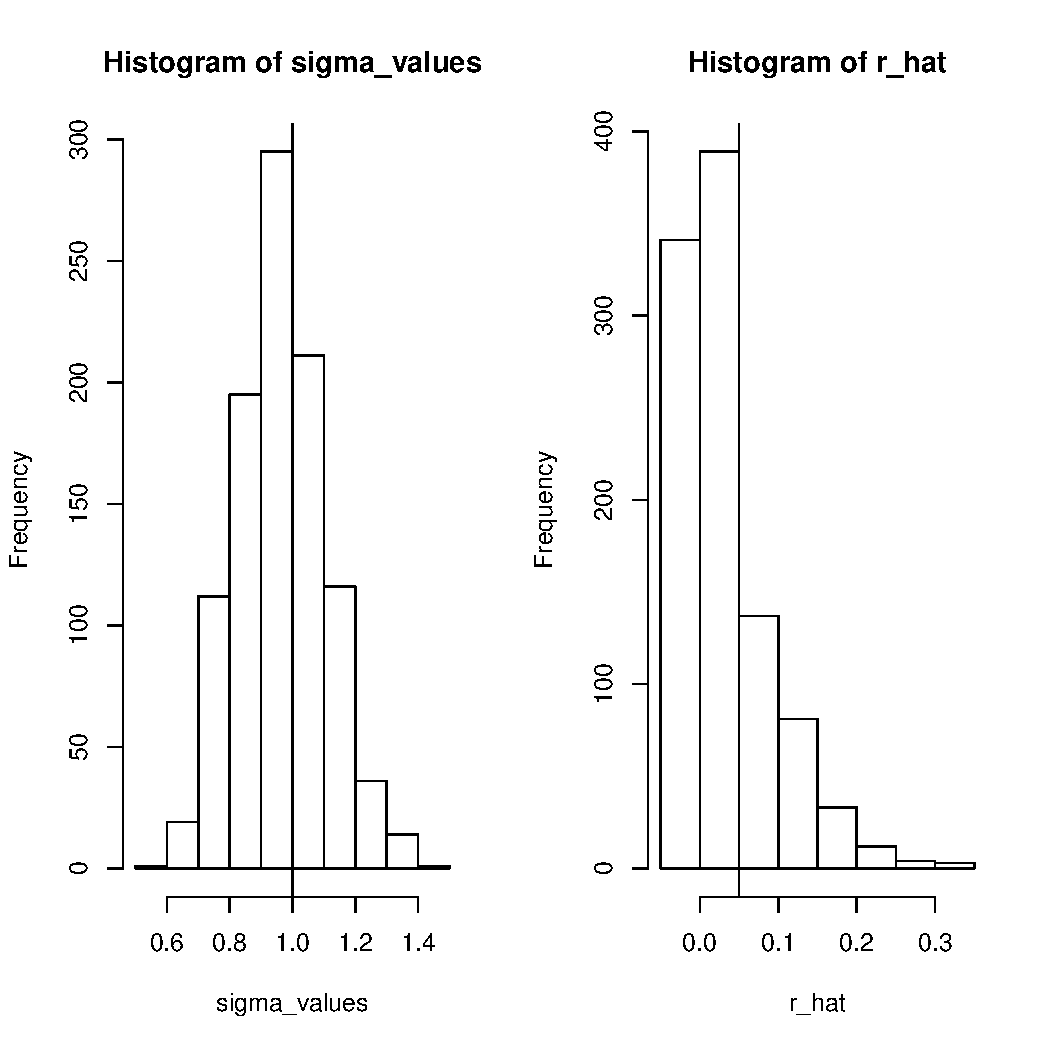
\includegraphics[width=\maxwidth]{figure/unnamed-chunk-1-1} 
\begin{kframe}\begin{alltt}
\hlkwd{par}\hlstd{(}\hlkwc{mfrow} \hlstd{=} \hlkwd{c}\hlstd{(}\hlnum{1}\hlstd{,}\hlnum{1}\hlstd{))}
\end{alltt}
\end{kframe}
\end{knitrout}

\begin{knitrout}
\definecolor{shadecolor}{rgb}{0.969, 0.969, 0.969}\color{fgcolor}\begin{kframe}
\begin{alltt}
\hlcom{# Relationship between var(Sn), r, sigma satisfied?}
\hlkwd{abs}\hlstd{(}\hlkwd{var}\hlstd{(S_n)}\hlopt{-}\hlstd{n}\hlopt{*}\hlstd{sigma_hat}\hlopt{^}\hlnum{2}\hlopt{-}\hlstd{n}\hlopt{*}\hlstd{(n}\hlopt{-}\hlnum{1}\hlstd{)}\hlopt{*}\hlstd{sigma_hat}\hlopt{^}\hlnum{2}\hlopt{*}\hlstd{r)}\hlopt{/}\hlkwd{var}\hlstd{(S_n)}
\end{alltt}
\begin{verbatim}
## [1] 0.1454494
\end{verbatim}
\begin{alltt}
\hlcom{# True value of S_n}
\hlstd{true_VarSn} \hlkwb{=} \hlstd{n}\hlopt{*}\hlnum{1}\hlopt{+}\hlstd{n}\hlopt{*}\hlstd{(n}\hlopt{-}\hlnum{1}\hlstd{)}\hlopt{*}\hlnum{1}\hlopt{*}\hlstd{r}
\hlstd{true_VarSn}
\end{alltt}
\begin{verbatim}
## [1] 595
\end{verbatim}
\begin{alltt}
\hlcom{# Relative error}
\hlkwd{abs}\hlstd{(true_VarSn}\hlopt{-} \hlkwd{var}\hlstd{(S_n))}\hlopt{/}\hlstd{true_VarSn}
\end{alltt}
\begin{verbatim}
## [1] 0.1907162
\end{verbatim}
\end{kframe}
\end{knitrout}

\subsection{OLS}

\begin{knitrout}
\definecolor{shadecolor}{rgb}{0.969, 0.969, 0.969}\color{fgcolor}\begin{kframe}
\begin{alltt}
\hlstd{X} \hlkwb{=} \hlkwd{matrix}\hlstd{(}\hlkwd{rnorm}\hlstd{(}\hlnum{100000}\hlstd{),}\hlnum{100}\hlstd{,}\hlnum{1000}\hlstd{)}
\hlstd{Y} \hlkwb{=} \hlstd{X} \hlopt{+} \hlstd{epsilons}

\hlstd{ols} \hlkwb{=} \hlkwa{function}\hlstd{(}\hlkwc{X}\hlstd{,}\hlkwc{Y}\hlstd{)\{}
  \hlstd{n} \hlkwb{=} \hlkwd{nrow}\hlstd{(X)}
  \hlstd{p} \hlkwb{=} \hlkwd{ncol}\hlstd{(X)}
  \hlstd{beta_hat_values} \hlkwb{=} \hlkwd{vector}\hlstd{(}\hlkwc{length} \hlstd{= p)}
  \hlstd{epsilon_values} \hlkwb{=} \hlkwd{matrix}\hlstd{(}\hlkwc{nrow} \hlstd{= n,} \hlkwc{ncol} \hlstd{= p)}
  \hlkwa{for} \hlstd{(i} \hlkwa{in} \hlnum{1}\hlopt{:}\hlstd{p)\{}
    \hlstd{Xi} \hlkwb{=} \hlstd{X[,i]}
    \hlstd{Yi} \hlkwb{=} \hlstd{Y[,i]}
    \hlstd{beta_hat_values[i]} \hlkwb{=} \hlkwd{solve}\hlstd{(}\hlkwd{t}\hlstd{(Xi)} \hlopt \hlstd{Xi)} \hlopt \hlkwd{t}\hlstd{(Xi)}\hlopt\hlstd{Yi}
    \hlstd{epsilon_values[,i]} \hlkwb{=} \hlstd{Yi}\hlopt{-}\hlstd{beta_hat_values[i]} \hlopt \hlstd{Yi}
  \hlstd{\}}
  \hlkwd{list}\hlstd{(}\hlkwc{beta_hat_values} \hlstd{= beta_hat_values,} \hlkwc{epsilons} \hlstd{= epsilon_values)}
\hlstd{\}}

\hlstd{beta_hat_values} \hlkwb{=} \hlkwd{ols}\hlstd{(X,Y)}\hlopt{$}\hlstd{beta_hat_values}

\hlcom{# Estimate of beta}
\hlkwd{mean}\hlstd{(beta_hat_values)}
\end{alltt}
\begin{verbatim}
## [1] 0.9997003
\end{verbatim}
\begin{alltt}
\hlkwd{hist}\hlstd{(beta_hat_values)}
\hlkwd{abline}\hlstd{(}\hlkwc{v} \hlstd{=} \hlnum{1}\hlstd{)}
\end{alltt}
\end{kframe}
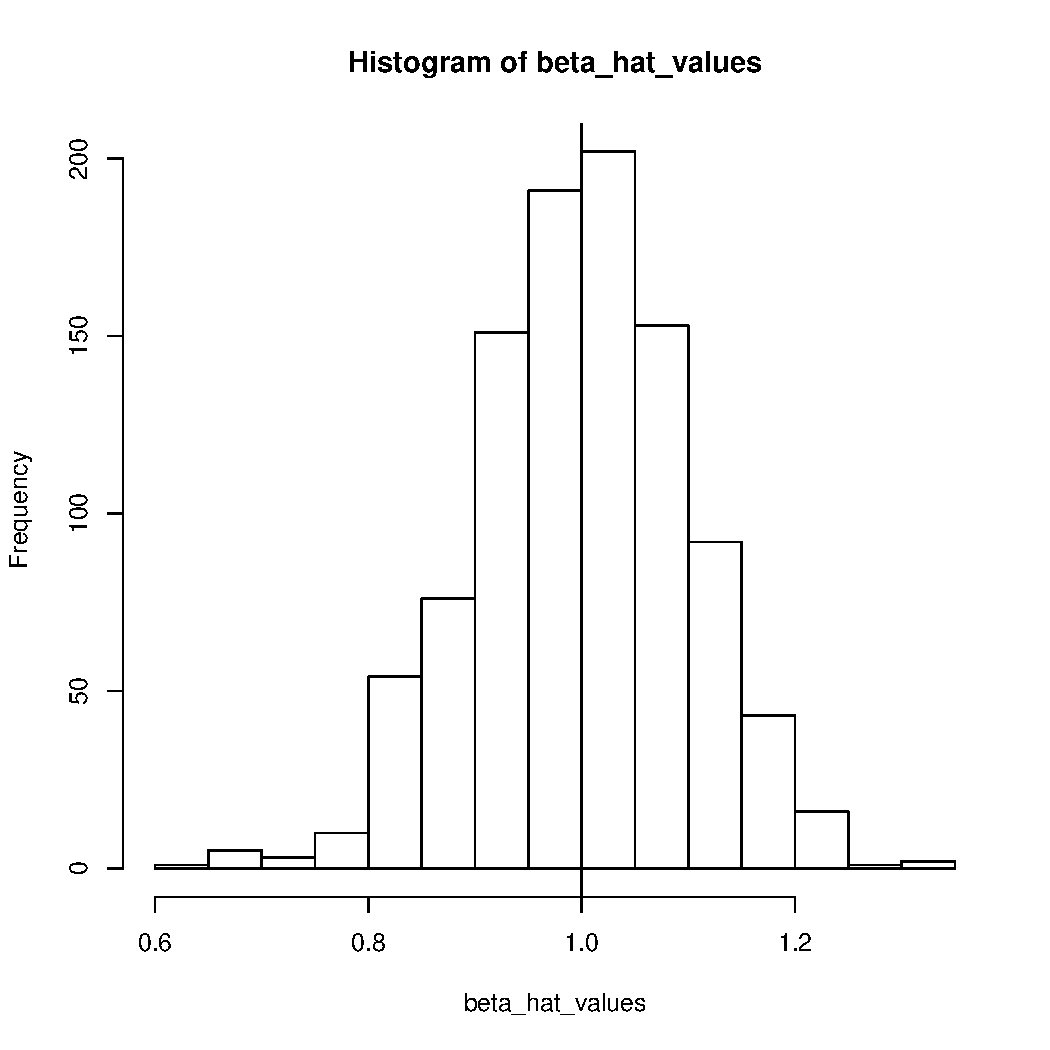
\includegraphics[width=\maxwidth]{figure/unnamed-chunk-3-1} 

\end{knitrout}
Here, OLS does pretty well since the estimatonr of $\beta$ is not biased and the variance is relatively low, as the histogram shows.

\subsection{One Step GLS}


\begin{knitrout}
\definecolor{shadecolor}{rgb}{0.969, 0.969, 0.969}\color{fgcolor}\begin{kframe}
\begin{alltt}
\hlstd{X} \hlkwb{=} \hlkwd{matrix}\hlstd{(}\hlkwd{rnorm}\hlstd{(}\hlnum{100000}\hlstd{),}\hlnum{100}\hlstd{,}\hlnum{1000}\hlstd{)}
\hlstd{Y} \hlkwb{=} \hlstd{X} \hlopt{+} \hlstd{epsilons}

\hlstd{gls} \hlkwb{=} \hlkwa{function}\hlstd{(}\hlkwc{X}\hlstd{,}\hlkwc{Y}\hlstd{,}\hlkwc{epsilons}\hlstd{,} \hlkwc{beta_hat_ols}\hlstd{)\{}
  \hlstd{n} \hlkwb{=} \hlkwd{nrow}\hlstd{(X)}
  \hlstd{p} \hlkwb{=} \hlkwd{ncol}\hlstd{(X)}
  \hlstd{non_diag_terms} \hlkwb{=} \hlstd{(}\hlkwd{matrix}\hlstd{(}\hlnum{1}\hlstd{,n,p)}\hlopt{-}\hlkwd{diag}\hlstd{(}\hlnum{1}\hlstd{,n,p))}\hlopt{>}\hlnum{0}
  \hlstd{beta_hat_values} \hlkwb{=} \hlstd{beta_hat_ols}
  \hlstd{var_hat_values} \hlkwb{=} \hlkwd{vector}\hlstd{(}\hlkwc{length} \hlstd{= p)}
  \hlstd{r_hat_values} \hlkwb{=} \hlkwd{vector}\hlstd{(}\hlkwc{length} \hlstd{= p)}
  \hlstd{epsilons_update} \hlkwb{=} \hlstd{epsilons}
  \hlkwa{for} \hlstd{(i} \hlkwa{in} \hlnum{1}\hlopt{:}\hlstd{p)\{}
    \hlcom{# Residuals}
    \hlstd{e} \hlkwb{=} \hlstd{Y[,i]} \hlopt{-} \hlstd{X[,i]}\hlopt{*}\hlstd{beta_hat_values[i]}
    \hlcom{# Empirical value of cov}
    \hlstd{cov_hat} \hlkwb{=} \hlstd{e} \hlopt \hlkwd{t}\hlstd{(e)}
    \hlcom{# Empirical value of var}
    \hlstd{var_hat_values[i]} \hlkwb{=} \hlkwd{mean}\hlstd{(}\hlkwd{diag}\hlstd{(cov_hat))}
    \hlcom{# Empirical value of r}
    \hlstd{r_hat_values[i]} \hlkwb{=} \hlkwd{mean}\hlstd{(cov_hat[}
      \hlkwd{lower.tri}\hlstd{(cov_hat,} \hlkwc{diag} \hlstd{=} \hlnum{FALSE}\hlstd{)]}\hlopt{/}\hlstd{var_hat_values[i])}
    \hlcom{# Estimate G}
    \hlstd{G_hat} \hlkwb{=} \hlkwd{matrix}\hlstd{(r_hat_values[i],n,n)} \hlopt{+}
      \hlkwd{diag}\hlstd{(var_hat_values[i]}\hlopt{-}\hlstd{r_hat_values[i],n,n)}
    \hlstd{G_hat_inv} \hlkwb{=} \hlkwd{solve}\hlstd{(G_hat)}
    \hlcom{# Add beta hat value}
    \hlstd{Xi} \hlkwb{=} \hlstd{X[,i]}
    \hlstd{Yi} \hlkwb{=} \hlstd{Y[,i]}
    \hlstd{beta_hat_values[i]} \hlkwb{=} \hlkwd{solve}\hlstd{(}\hlkwd{t}\hlstd{(Xi)} \hlopt \hlstd{G_hat_inv} \hlopt \hlstd{Xi)} \hlopt
      \hlkwd{t}\hlstd{(Xi)} \hlopt \hlstd{G_hat_inv} \hlopt \hlstd{Yi}
    \hlcom{# Update epsilon}
    \hlstd{epsilons_update[,i]} \hlkwb{=} \hlstd{G_hat_inv} \hlopt \hlstd{e}
  \hlstd{\}}
  \hlkwd{return}\hlstd{(}\hlkwd{list}\hlstd{(}\hlkwc{beta_hat_values} \hlstd{= beta_hat_values,}
              \hlkwc{epsilons} \hlstd{= epsilons_update,}
              \hlkwc{r_hat_values} \hlstd{= r_hat_values,}
              \hlkwc{var_hat_values} \hlstd{= var_hat_values))}
\hlstd{\}}

\hlstd{beta_hat_ols} \hlkwb{=} \hlkwd{ols}\hlstd{(X,Y)}\hlopt{$}\hlstd{beta_hat_values}
\hlstd{gls_out} \hlkwb{=} \hlkwd{gls}\hlstd{(X,Y,epsilons,beta_hat_ols)}
\end{alltt}
\end{kframe}
\end{knitrout}
Here, we see that the estimators of $\beta$, $\sigma$ and $r$ are not biased. For $\beta$, we can say that the estimator is as good as the OLS.
\begin{knitrout}
\definecolor{shadecolor}{rgb}{0.969, 0.969, 0.969}\color{fgcolor}\begin{kframe}
\begin{alltt}
\hlkwd{par}\hlstd{(}\hlkwc{mfrow} \hlstd{=} \hlkwd{c}\hlstd{(}\hlnum{1}\hlstd{,}\hlnum{3}\hlstd{))}
\hlcom{# Estimate of beta}
\hlstd{beta_hat_values} \hlkwb{=} \hlstd{gls_out}\hlopt{$}\hlstd{beta_hat_values}
\hlkwd{mean}\hlstd{(beta_hat_values)}
\end{alltt}
\begin{verbatim}
## [1] 1.001561
\end{verbatim}
\begin{alltt}
\hlkwd{hist}\hlstd{(beta_hat_values)}
\hlkwd{abline}\hlstd{(}\hlkwc{v} \hlstd{=} \hlnum{1}\hlstd{)}

\hlcom{# Empirical value of sigma}
\hlstd{sigma_values} \hlkwb{=} \hlkwd{sqrt}\hlstd{(gls_out}\hlopt{$}\hlstd{var_hat_values)}
\hlkwd{mean}\hlstd{(sigma_values)}
\end{alltt}
\begin{verbatim}
## [1] 0.9923265
\end{verbatim}
\begin{alltt}
\hlkwd{hist}\hlstd{(sigma_values)}
\hlkwd{abline}\hlstd{(}\hlkwc{v} \hlstd{=} \hlnum{1}\hlstd{)}

\hlcom{# Empirical value of r}
\hlstd{r_values} \hlkwb{=} \hlstd{gls_out}\hlopt{$}\hlstd{r_hat_values}
\hlkwd{mean}\hlstd{(r_values)}
\end{alltt}
\begin{verbatim}
## [1] 0.03493974
\end{verbatim}
\begin{alltt}
\hlkwd{hist}\hlstd{(r_values)}
\hlkwd{abline}\hlstd{(}\hlkwc{v} \hlstd{= r)}
\end{alltt}
\end{kframe}
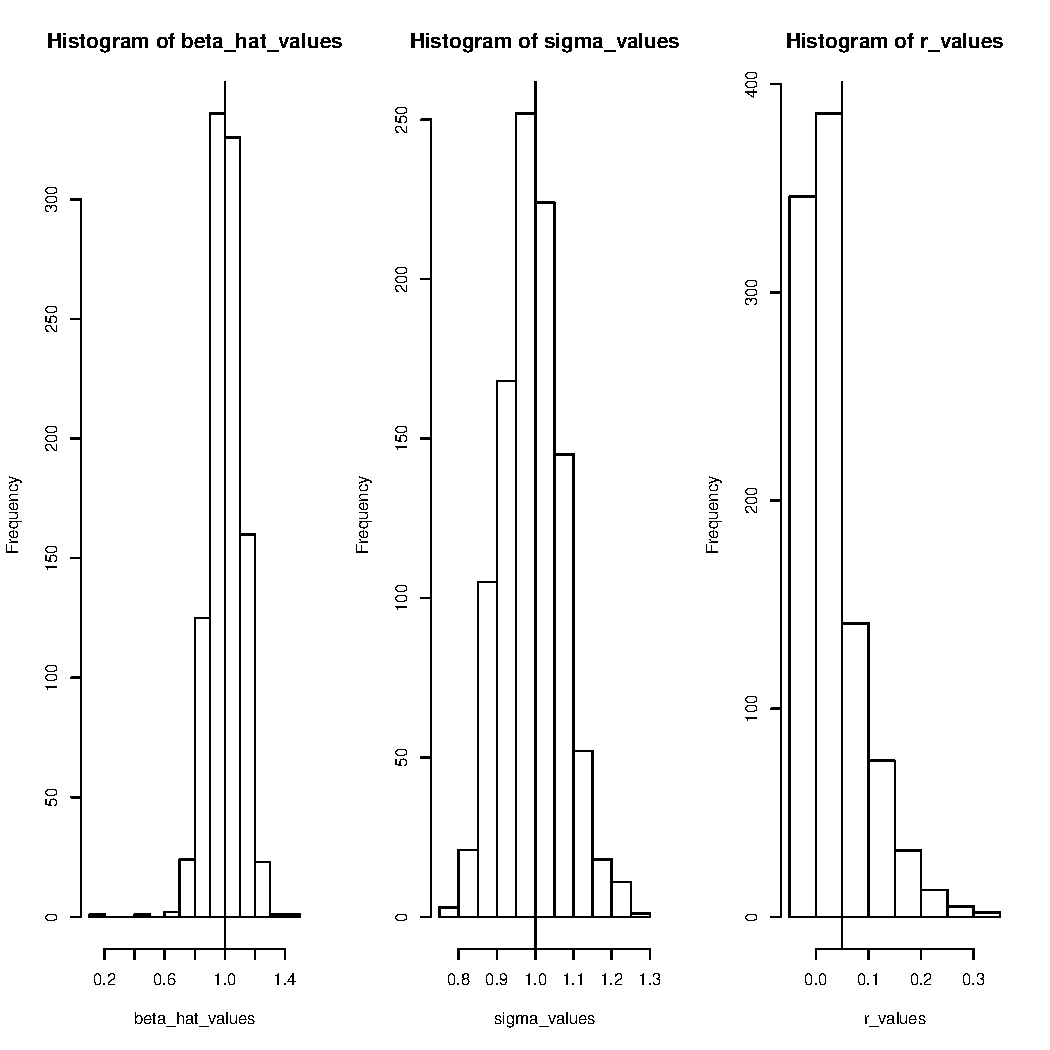
\includegraphics[width=\maxwidth]{figure/unnamed-chunk-5-1} 
\begin{kframe}\begin{alltt}
\hlkwd{par}\hlstd{(}\hlkwc{mfrow} \hlstd{=} \hlkwd{c}\hlstd{(}\hlnum{1}\hlstd{,}\hlnum{1}\hlstd{))}
\end{alltt}
\end{kframe}
\end{knitrout}


\subsection{Five Step GLS}

\begin{knitrout}
\definecolor{shadecolor}{rgb}{0.969, 0.969, 0.969}\color{fgcolor}\begin{kframe}
\begin{alltt}
\hlcom{### 4. Five Step GLS}

\hlstd{gls_it} \hlkwb{=} \hlkwa{function}\hlstd{(}\hlkwc{X}\hlstd{,}\hlkwc{Y}\hlstd{,}\hlkwc{n_it}\hlstd{)\{}
  \hlcom{# Step zero: ols}
  \hlstd{ols_out} \hlkwb{=} \hlkwd{ols}\hlstd{(X,Y)}
  \hlstd{epsilons_update} \hlkwb{=} \hlstd{ols_out}\hlopt{$}\hlstd{epsilons}
  \hlstd{beta_hat_update} \hlkwb{=} \hlstd{ols_out}\hlopt{$}\hlstd{beta_hat_values}
  \hlcom{# Iterations}
  \hlstd{beta_hat_values_it} \hlkwb{=} \hlkwd{matrix}\hlstd{(}\hlkwc{nrow} \hlstd{=} \hlnum{1000}\hlstd{,} \hlkwc{ncol} \hlstd{= n_it)}
  \hlstd{var_hat_values_it} \hlkwb{=} \hlkwd{matrix}\hlstd{(}\hlkwc{nrow} \hlstd{=} \hlnum{1000}\hlstd{,} \hlkwc{ncol} \hlstd{= n_it)}
  \hlstd{r_hat_values_it} \hlkwb{=} \hlkwd{matrix}\hlstd{(}\hlkwc{nrow} \hlstd{=} \hlnum{1000}\hlstd{,} \hlkwc{ncol} \hlstd{= n_it)}
  \hlkwa{for} \hlstd{(j} \hlkwa{in} \hlnum{1}\hlopt{:}\hlstd{n_it)\{}
    \hlstd{gls_out} \hlkwb{=} \hlkwd{gls}\hlstd{(X,Y,epsilons_update,beta_hat_update)}
    \hlstd{beta_hat_values_it[,j]} \hlkwb{=} \hlstd{gls_out}\hlopt{$}\hlstd{beta_hat_values}
    \hlstd{var_hat_values_it[,j]} \hlkwb{=} \hlstd{gls_out}\hlopt{$}\hlstd{var_hat_values}
    \hlstd{r_hat_values_it[,j]} \hlkwb{=} \hlstd{gls_out}\hlopt{$}\hlstd{r_hat_values}
    \hlstd{epsilons_update} \hlkwb{=} \hlstd{gls_out}\hlopt{$}\hlstd{epsilons}
    \hlstd{beta_hat_update} \hlkwb{=} \hlstd{beta_hat_values_it[,j]}
    \hlkwd{cat}\hlstd{(}\hlstr{'Step '}\hlstd{,j,}\hlstr{' done.\textbackslash{}n'}\hlstd{)}
  \hlstd{\}}
  \hlkwd{list}\hlstd{(}\hlkwc{beta_hat_values_it} \hlstd{= beta_hat_values_it,}
       \hlkwc{var_hat_values_it} \hlstd{= var_hat_values_it,}
       \hlkwc{r_hat_values_it} \hlstd{= r_hat_values_it)}
\hlstd{\}}
\hlstd{gls_it_out} \hlkwb{=} \hlkwd{gls_it}\hlstd{(X,Y,}\hlnum{5}\hlstd{)}
\end{alltt}
\begin{verbatim}
## Step  1  done.
## Step  2  done.
## Step  3  done.
## Step  4  done.
## Step  5  done.
\end{verbatim}
\begin{alltt}
\hlstd{beta_hat_values_it} \hlkwb{=} \hlstd{gls_it_out}\hlopt{$}\hlstd{beta_hat_values_it}
\hlstd{var_hat_values_it} \hlkwb{=} \hlstd{gls_it_out}\hlopt{$}\hlstd{var_hat_values_it}
\hlstd{r_hat_values_it} \hlkwb{=} \hlstd{gls_it_out}\hlopt{$}\hlstd{r_hat_values_it}

\hlkwd{boxplot}\hlstd{(beta_hat_values_it,} \hlkwc{main} \hlstd{=} \hlstr{"Five Step GLS"}\hlstd{,}
        \hlkwc{xlab} \hlstd{=} \hlstr{"Iterations"}\hlstd{,} \hlkwc{ylab} \hlstd{=} \hlstr{"Beta estimation"}\hlstd{,}
        \hlkwc{range}\hlstd{=}\hlnum{0}\hlstd{)}
\hlkwd{abline}\hlstd{(}\hlkwc{h}\hlstd{=}\hlnum{1}\hlstd{)}
\end{alltt}
\end{kframe}
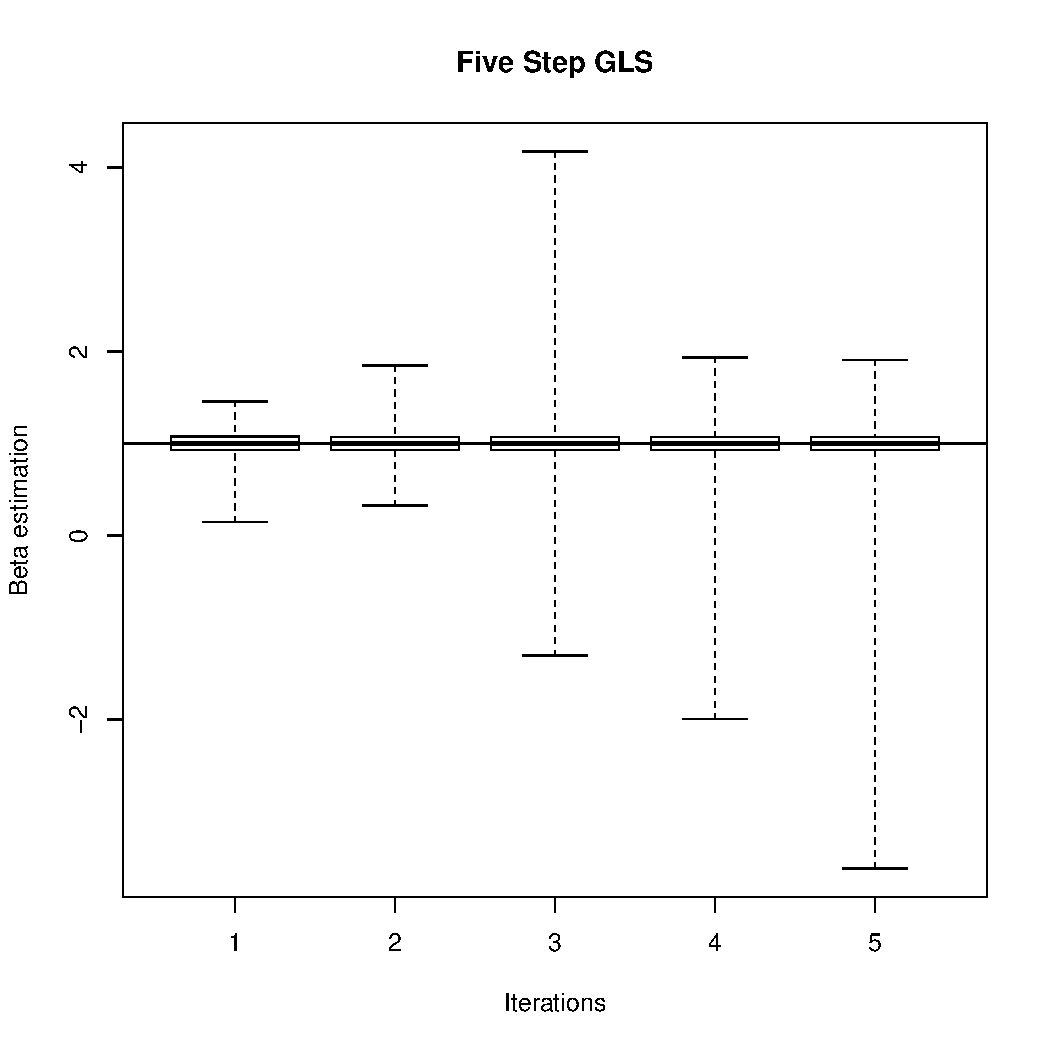
\includegraphics[width=\maxwidth]{figure/unnamed-chunk-6-1} 
\begin{kframe}\begin{alltt}
\hlkwd{par}\hlstd{(}\hlkwc{mfrow} \hlstd{=} \hlkwd{c}\hlstd{(}\hlnum{1}\hlstd{,}\hlnum{3}\hlstd{))}
\hlcom{# Estimate of beta}
\hlstd{beta_hat_values} \hlkwb{=} \hlstd{beta_hat_values_it[,}\hlnum{5}\hlstd{]}
\hlkwd{mean}\hlstd{(beta_hat_values)}
\end{alltt}
\begin{verbatim}
## [1] 0.9913742
\end{verbatim}
\begin{alltt}
\hlkwd{hist}\hlstd{(beta_hat_values)}
\hlkwd{abline}\hlstd{(}\hlkwc{v} \hlstd{=} \hlnum{1}\hlstd{)}

\hlcom{# Empirical value of sigma}
\hlstd{sigma_values} \hlkwb{=} \hlkwd{sqrt}\hlstd{(var_hat_values_it[,}\hlnum{5}\hlstd{])}
\hlstd{sigma_hat} \hlkwb{=} \hlkwd{mean}\hlstd{(sigma_values)}
\hlstd{sigma_hat}
\end{alltt}
\begin{verbatim}
## [1] 0.996248
\end{verbatim}
\begin{alltt}
\hlkwd{hist}\hlstd{(sigma_values)}
\hlkwd{abline}\hlstd{(}\hlkwc{v} \hlstd{=} \hlnum{1}\hlstd{)}

\hlcom{# Empirical value of r}
\hlstd{r_values} \hlkwb{=} \hlstd{r_hat_values_it[,}\hlnum{5}\hlstd{]}
\hlstd{r_hat} \hlkwb{=} \hlkwd{mean}\hlstd{(r_values)}
\hlstd{r_hat}
\end{alltt}
\begin{verbatim}
## [1] 0.03568166
\end{verbatim}
\begin{alltt}
\hlkwd{hist}\hlstd{(r_values)}
\hlkwd{abline}\hlstd{(}\hlkwc{v} \hlstd{= r)}
\end{alltt}
\end{kframe}
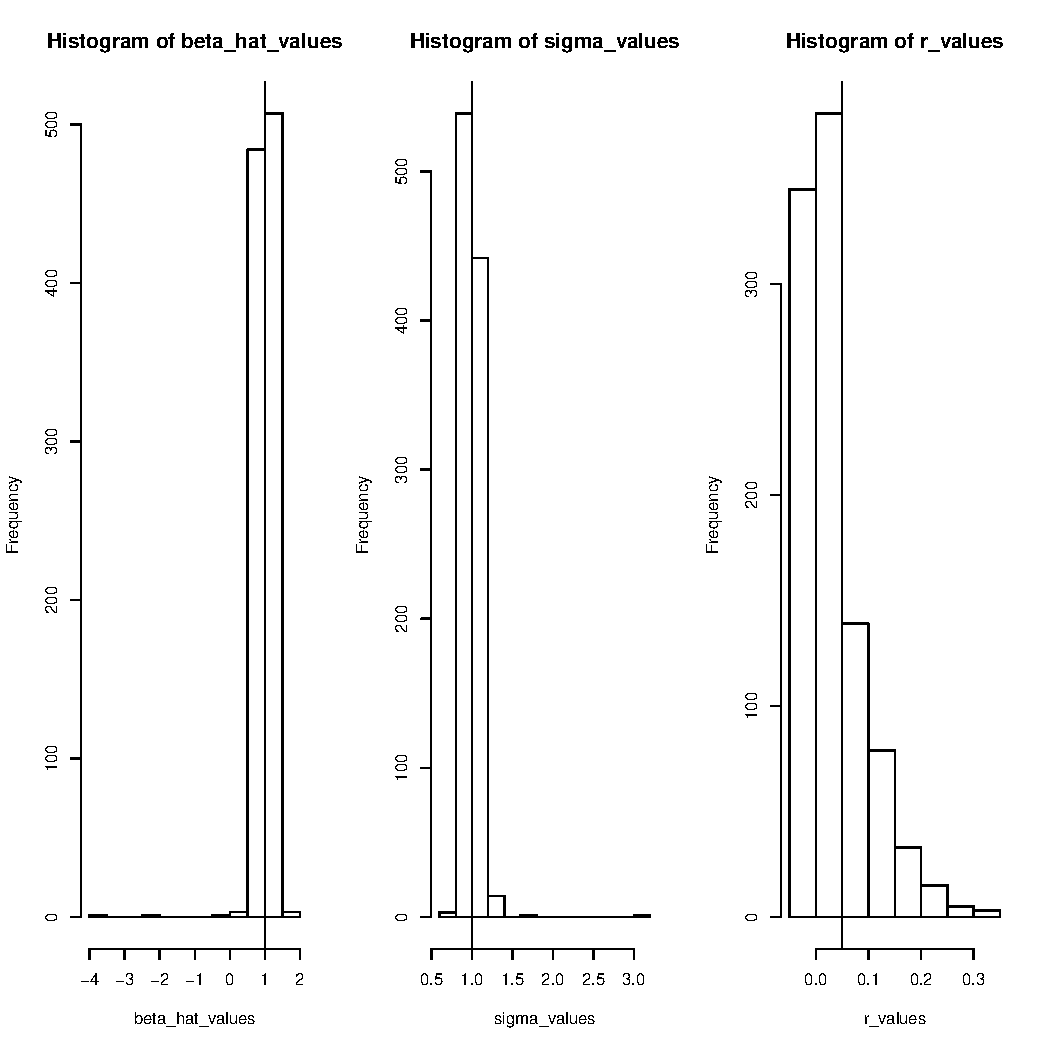
\includegraphics[width=\maxwidth]{figure/unnamed-chunk-6-2} 
\begin{kframe}\begin{alltt}
\hlkwd{par}\hlstd{(}\hlkwc{mfrow} \hlstd{=} \hlkwd{c}\hlstd{(}\hlnum{1}\hlstd{,}\hlnum{1}\hlstd{))}
\end{alltt}
\end{kframe}
\end{knitrout}
Here, the estimate is unbiased, and we see that the first estimation gives pretty accurate results. Moreover, the 5 steps make no improvement. We have more extreme values at the fith step than at the first one. It makes sense because here the $G$ matrix is highly constrained and by updating it we allow more variance in the estimate.
\end{document}









